\providecommand{\main}{../../../..}
\documentclass[\main/dresen_thesis.tex]{subfiles}

\begin{document}
  \paragraphNewLine{Transmission Electron Microscopy}
    Micrographs from transmission electron microscopy were obtained by the collaboration from the University of Mainz that prepared the nanoparticles.
    The micrographs were measured on a FEI Tecnai T-12-TEM with \ch{LaB6} cathode at an acceleration voltage of $120 \unit{kV}$.
    The nanosphere diameter and size distributio of over 200 nanoparticles was measured manually using the Fiji distribution \cite{Schindelin_2012_Fijia} and evaluated by fitting a log-normal distribution as described in \refch{ch:methods:em}.

    Due to the occurence of a large asymmetric size distribution in one batch, it is necessary to fit a bimodal log-normal distribution to properly describe the observed probability distribution.
    The bimodal distribution is defined by
    \begin{align}
      p_\mathrm{bimodal}(d) \eq \alpha p_1(d; \mu_1, \sigma_1) + (1 - \alpha) p_2(d; \mu_2, \sigma_2),
    \end{align}
    where $\alpha$ is the fraction of the first mode, $\mu_1$, $\sigma_1$ the log-normal parameters for the first mode and $\mu_2$, $\sigma_2$ the parameters for the second mode.

  \paragraphNewLine{X-Ray Diffraction}
    X-ray diffraction of IOS-11 was measured in cooperation with the group of Daniel Nižňanský from the Department of Inorganic Chemistry at the Charles University in Prague on an PANanalytical X'Pert PRO, which is described in \refch{ch:instruments:laboratoryInstruments:xrd}.
    The sample was dried for the transport and redispersed at the laboratory in Prague where it was then evaporated on a glass substrate for the measurement.
    The experiment was performed with a Cu-K$\alpha$ source ($\lambda \eq 1.54 \angstrom$) and a $2 \theta \eq 5^\circ \ldots 80^\circ$ has been measured.
    The instrumental broadening is determined from a LaB6 reference measurement (SR 660b, NIST).

    To evaluate the data, a LeBail fit is performed using the FullProf suite \cite{Rodriguez_1993_Recen} as described in \refch{ch:methods:xrd}.
    The background was estimated manually by selecting around 20 background points, from which the measured range is interpolated linearly.
    Due to a large background coming from the glass substrate at low angles, the data between $5 ^\circ \ldots 15 ^\circ$ is excluded from the refinement.
    As it is shown that the inverse spinell phase (space group $Fd\bar{3}m$, No. 227) of magnetite/maghemite is not sufficient to describe the XRD, a combination of an inverse spinell phase and a w\"ustite phase (space group $Fm\bar{3}m$, No. 225) is refined.

  % \paragraphNewLine{Energy-Dispersive X-Ray Spectroscopy}
  %   By using the scanning electron microscope Neon Zeiss 40 (\refch{ch:instruments:laboratoryInstruments:sem}) in EDX mode, it is confirmed for both nanoparticle batches that they only the characteristic signatures of iron, carbon and oxygen are visible and no elemental impurities are present.

  \paragraphNewLine{Small-Angle Scattering}
    Dispersions of IOS-11 and IOS-7 were measured using SAXS at GALAXI (\refch{ch:lss:galaxi}) and SANS(POL) at D33 (\refch{ch:lss:d33}) to determine the electronic, nuclear and magnetic structure of the nanospheres.

    For the SAXS measurement, the dispersions are filled in borosilicate capillaries (Hilgenberg) with $1.5 \unit{mm}$ diameter and a $0.01 \unit{mm}$ wall thickness.
    The capillaries are sealed vacuum-tight on top with a plastic stopper and a liquid glue that cures under UV light (Norland Optical Adhesive).
    Both samples are dispersed in cyclohexane for the measurement.
    The used solvents and concentrations are given in \reftab{tab:monolayers:charMethod:sampleConcentrations}.
    The samples are measured on the largest ($3.53 \unit{m}$) and shortest ($0.83 \unit{m}$) sample-to-detector distances possible at GALAXI at the Ga-K$\alpha$ wavelength of $\lambda \eq 1.3414 \angstrom$.
    Additionally, a capillary filled with cyclohexane and an empty capillary is measured under the same conditions for subtraction of the background.
    The SAXS data is scaled to absolute units according to the procedure described in \refch{ch:methods:saxs}.

    \begin{table}[!htbp]
      \centering
      \caption{\label{tab:monolayers:charMethod:sampleConcentrations}Solvents and gravimetric concentrations $c_m$ for samples measured in SAXS and SANS.}
      \begin{tabular}{ l | l | c | l | c }
        \textbf{Sample}  & Solvent (SAXS) & $c_m^\mathrm{SAXS} \,/ \unit{gL^{-1}}$ & Solvent (SANS) & $c_m^\mathrm{SANS}\,/ \unit{gL^{-1}}$\\
        \hline
        IOS-11 & cyclohexane   &                  & toluene-d8       & 2.8\\
        IOS-7  & cyclohexane   &                  & toluene-d8       & 2.0\\
        \hline
      \end{tabular}
    \end{table}


    For the SANSPOL measurement on the D33 instrument, $500 \unit{\musf L}$ of the IOS-11 and $250 \unit{\musf L}$ of the IOS-7 stock solution is dried over night at ambient conditions, and then redispersed in $1 \unit{mL}$ of toluene-$\mathrm{d_8}$ by sonification.
    The dispersions are measured in Hellma quartz cuvettes with a thickness of $2 \unit{mm}$.
    The wavelength at D33 was set to $6 \unit{\angstrom}$, where the selector provides a wavelength spread of $10 \%$ (FWHM).
    A sample aperture  of $7 \times 10 \unit{mm^2}$ was used and a collimation aperture of $30 \times 30 \unit{mm^2}$ is set for all experiments.
    The samples are measured both at a sample-to-detector distance of $2 \unit{m}$ and at $8 \unit{m}$ with a collimation distance of $5.3 \unit{m}$ and $7.8 \unit{m}$ respectively.
    The nanoparticles are measured at an magnetic field of $515 \unit{mT}$, which is applied perpendicular to the beam direction, in the horizontal direction.
    Each sample is measured over a time of $20 \unit{min}$ at the long sample-to-detector distance and $10 \unit{min}$ at the short sample-to-detector distance.
    The empty beam and a sample of toluene-$\mathrm{d_8}$ is measured 
    For the evaluation of the magnetic scattering, a $20^\circ$ sector around the vertical dimension is azimuthally integrated by using the GRASP software.
    Furthermore, the polarization efficiency of $97 \%$ and a flipping efficiency of $99 \%$ of D33, according to the instrument specifications given by the local contact, is corrected with the GRASP software during data reduction.

    From the distances and aperture sizes, an angular divergence of $2.1 \unit{mrad}$ and $3.8 \unit{mrad}$ are calculated for the long and short detector distance respectively by \refeq{eq:methods:sans:formulaResolution}, which is fixed together with the wavelength spread for the data evaluation.

    To evaluate the SAXS data, a spherical core-shell form factor is assumed with a w\"ustite core and a maghemite shell.
    The scattering length density of the core and shell material is calculated by
    \begin{align}
      \rho^\mathrm{X-ray}_\mathrm{maghemite}   &\eq   \frac{32 r_e}{3}  \frac{2 f_\mathrm{Fe} + 3 f_\mathrm{O}}
                                                                  {a_\mathrm{maghemite}^3}
                                                \eq & 38.56 \cdot 10^{-6} \angstrom^{-2},\\
      \rho^\mathrm{neutron}_\mathrm{maghemite} &\eq   \frac{32}{3} \frac{2 b_\mathrm{Fe} + 3 b_\mathrm{O}}
                                                                  {a_\mathrm{maghemite}^3}
                                                \eq & 6.57 \cdot 10^{-6} \angstrom^{-2},\\
      \rho^\mathrm{X-ray}_\textsf{w\"ustite}   &\eq   4 r_e \frac{f_\mathrm{Fe} + f_\mathrm{O}}
                                                                  {a_\textsf{w\"ustite}^3}
                                                \eq & 52.07 \cdot 10^{-6} \angstrom^{-2},\\
      \rho^\mathrm{neutron}_\textsf{w\"ustite} &\eq   4 \frac{b_\mathrm{Fe} + b_\mathrm{O}}
                                                              {a_\textsf{w\"ustite}^3}
                                                \eq & 8.34 \cdot 10^{-6} \angstrom^{-2}.
    \end{align}
    with $r_e$ the classical electron radius, the  atomic form factor $f$ and nuclear coherent scattering length $b$ of iron and oxygen, both are found in literature for the elements of the periodic table and are tabulated for iron and oxygen in \reftab{tab:looselyPackedNS:charMethod:scatteringLenghts}.
    The lattice constants are estimated from the values that are obtained in XRD for IOS-11.
    \begin{table}[ht]
      \centering
      \caption{\label{tab:looselyPackedNS:charMethod:scatteringLenghts}Atomic form factor $f$ (at $\lambda \eq 1.3414 \unit{\angstrom}$) and the nuclear coherent scattering length $b$ of iron and oxygen \cite{Sears_1992_Neutr, BerkeleyLab_1993_asf}.}
      \begin{tabular}{ c | l | c }
                  & $f$       & $b \, / \unit{fm}$ \\
        \hline
        $\ch{O}$  & 8.04077   & 5.803   \\
        $\ch{Fe}$ & 25.7468   & 9.45  \\
        \hline
      \end{tabular}
    \end{table}

    The SLD of the surfactant oleic acid is calculated from literature
    \begin{align}
      \rho^\mathrm{X-ray}_\mathrm{oleic\,acid} &\eq 8.52 \cdot 10^{-6} \angstrom^{-2},\\
      \rho^\mathrm{neutron}_\mathrm{oleic\,acid} &\eq 0.078 \cdot 10^{-6} \angstrom^{-2},
    \end{align}
    which assumes a density of $0.895 \unit{g\,mL^{-1}}$ for the oleic acid.
    As well as the solvent scattering length densities, which are fixed to the values calculated from literature
    \begin{align}
      \rho^\mathrm{X-ray}_{\mathrm{cyclohexane}} &\eq 7.55 \cdot 10^{-6} \angstrom^{-2},\\
      \rho^\mathrm{neutron}_\mathrm{toluene-d8}  &\eq 5.66 \cdot 10^{-6} \angstrom^{-2},
    \end{align}
    where a density of $0.779 \unit{g\,mL^{-1}}$ for cyclohexane, and $0.943 \unit{g\,mL^{-1}}$ for toluene-d8.

    In the minimization procedure of both SAXS and SANS models, a Levenberg-Marquardt algorithm\cite{Marquardt_1963_Analgo, Oliphant_2006_Guide} is applied for which a modified $\chi^2$ on the logarithmic scale is used
    \begin{align}
      \chi^2 \eq \frac{1}{N-p} \sum_{i\eq 1}^{N} \frac{(\log(I_i) - \log(I_\mathrm{model}))^2}{\sigma_i^2} I^2_i.
    \end{align}

    Furthermore, as the particle size and size distribution is very well determined by SAXS, which has a larger dynamic range in scattering vector, these parameters are not varied for the SANS form factor, where vice-versa the surfactant thickness is only determined by SANS and then fixed in the SAXS form factor.
    This is done until both calculated form factors are self-consistent with each other.
    However, the shell thickness of the maghemite phase is allowed to vary independently for both SAXS and SANS, as both experiments are sensitive to the shell thickness and as the SANS particles might have oxidized differently to the SAXS particles due to the solvent changing, where the particles were dry for a night at ambient conditions.

    The obtained particle number density $n$ obtained as parameter from SAS, is transformed to a mass concentration of the particles by
    \begin{align}
      c_m \eq n (\rho_\textsf{w\"ustite} V_p^\textsf{w\"ustite} + \rho_\textsf{maghemite} V_p^\textsf{maghemite}),
    \end{align}
    where $V^x_p$ is the average volume of the respective phase $x$ in a single nanosphere and $\rho$ the mass density of w\"ustite and maghemite that is determined from XRD.

%     8.3842688
% 4.1819711



  %   The numerical value $8$ accounts that one unit cell contains eight formula units of $\ch{Co_xFe_yO4}$ in an inverse spinell phase.
  %   The atomic form factor depends on the X-ray wavelength, the given values are for the wavelength of $\lambda \eq 1.3414 \unit{\angstrom}$ (wavelength used at the GALAXI instrument).
  %   For Ac-CoFe-C-3 no XRD was performed and therefore the literature value of the lattice constant is assumed.
  %   \begin{table}[ht]
  %     \centering
  %     \caption{\label{tab:monolayers:charMethod:scatteringLenghts}The real part of the atomic form factor $f$ (at $\lambda \eq 1.3414 \unit{\angstrom}$) and the nuclear coherent scattering length $b$ for the elements of the nanoparticles to determine their scattering length densities \cite{Sears_1992_Neutr, BerkeleyLab_1993_asf}.}
  %     \begin{tabular}{ c | l | c }
  %                 & $f$       & $b \, / \unit{fm}$ \\
  %       \hline
  %       $\ch{O}$  & 8.04077   & 5.803   \\
  %       $\ch{Co}$ & 26.3717   & 2.49  \\
  %       $\ch{Fe}$ & 25.7468   & 9.45  \\
  %       \hline
  %     \end{tabular}
  %   \end{table}

  %   For Ol-CoFe-C the superball form factor is used with an additional core-shell structure to account for the w\"ustite / inverse spinell structure of the particles and to determine the shell scattering length density $\rho_\mathrm{shell}$ and shell thickness $D_\mathrm{shell}$.
  %   For the SANS models, an additional oleic acid surfactant shell with the same superball parameters as the core model and a thickness $D_\mathrm{OA}$ is added to the model, which is neglected for SAXS models due to the poor contrast of oleic acid and solvent.
  %   However, the composition of the core and shell can not be determined by XRD and EDX alone as the complex structure leaves too many variables.
  %   There is luckily a significant contrast between the w\"ustite SLD ($\rho_\mathrm{el}^\textsf{w\"ustite} \approx 50 \cdot 10^{-6} \angstrom^{-2}$) and inverse spinell SLD ($\rho_\mathrm{el}^\mathrm{inv.\, spinell} \approx 42 \cdot 10^{-6} \angstrom^{-2}$) for X-rays, that enables to determine the relative core and shell thickness.
  %   And furthermore neutrons are highly sensitive to the relative iron and cobalt amount in a phase, as can be seen from \reftab{tab:monolayers:charMethod:scatteringLenghts}, which can be utilized to measure the relative composition.
  %   Thus the combination of SAXS and SANS can be used as a tool to solve both the core-shell structure and the compositions.

  %   The model for Ol-CoFe-C is therefore given a parameter for the cobalt content $x$ from the cobalt ferrite shell \ch{Co_x Fe_{3-x} O4}.
  %   Using this parameter, the scattering length density of the core and shell in Ol-CoFe-C is determined as described in the following:
  %   Fixing the ratio of iron and cobalt $r$ to the value obtained from EDX, the composition of the w\"ustite phase \ch{Fe_y Co_{1-y} O} is calculated using the volume of the spinell phase $V_\mathrm{inv.\,spinell}$ and the volume of the w\"ustite phase $V_\textsf{w\"ustite}$ in the core-shell particle, as well as the lattice constants determined from XRD $a_\mathrm{inv.\,spinell}$ and $a_\textsf{w\"ustite}$ by
  %   \begin{align}
  %     \begin{split}
  %       r &\eq \frac{N_\mathrm{Fe}^\mathrm{inv.\, spinell} + N_\mathrm{Fe}^\textsf{w\"ustite}}
  %                   {N_\mathrm{Co}^\mathrm{inv.\, spinell} + N_\mathrm{Co}^\textsf{w\"ustite}} \\
  %         &\eq \frac
  %               {8 (3-x) \frac{V_\mathrm{inv.\,spinell}}{a_\mathrm{inv.\,spinell}^3} +
  %                 4 y \frac{V_\textsf{w\"ustite}}{a_\textsf{w\"ustite}^3}}
  %               {8 x \frac{V_\mathrm{inv.\,spinell}}{a_\mathrm{inv.\,spinell}^3} +
  %                 4 (1-y) \frac{V_\textsf{w\"ustite}}{a_\textsf{w\"ustite}^3}}.
  %     \end{split}
  %   \end{align}
  %   This equation is straight forward to solve for $y$ by
  %   \begin{align}
  %     y &\eq \frac{2}{\nu} x + \frac{r \nu - 6}{\nu (1 + r)},\\
  %       & \textsf{where\,} \hspace{0.5cm} \nu \eq \frac{V_\textsf{w\"ustite}}{V_\mathrm{inv.\,spinell}} \biggl( \frac{a_\mathrm{inv.\,spinell}}{a_\textsf{w\"ustite}} \biggr)^3.
  %   \end{align}
  %   The volumes of the two phases are determined from the particle size, shell thickness and superball exponent on the fly during the fitting process, such that y is readily determined with varied particle dimensions and cobalt content in \ch{Co_x Fe_{3-x}O4}.
  %   % As SAXS is also sensitive to the difference of the nanoparticle core and shell size due to a stronger contrast between w\"ustite and spinell phase, the data sets for SAXS and SANS are fitted simultaneously.
  %   By this method, the combination of SAXS and SANS on Ol-CoFe-C provides the means to determine the particle size and size distribution, the individual core and shell thickness and atomic composition of the two phases, while being self-consistent with EDX and XRD results.

  %   The scattering length density of the oleic acid shell is fixed in every SANS model to the value value calculated for bulk oleic acid
  %   \begin{align}
  %     \rho^\mathrm{X-ray}_\mathrm{oleic\,acid} &\eq 8.52 \cdot 10^{-6} \angstrom^{-2},\\
  %     \rho^\mathrm{neutron}_\mathrm{oleic\,acid} &\eq 0.078 \cdot 10^{-6} \angstrom^{-2},
  %   \end{align}
  %   which assumes a density of $0.895 \unit{g\,mL^{-1}}$ for the oleic acid.
  %   The solvent scattering length densities are fixed to the values calculated from literature
  %   \begin{align}
  %     \rho^\mathrm{X-ray}_{n\mathrm{-hexane}}    &\eq 6.46 \cdot 10^{-6} \angstrom^{-2},\\
  %     \rho^\mathrm{X-ray}_\mathrm{toluene}       &\eq 8.01 \cdot 10^{-6} \angstrom^{-2},\\
  %     \rho^\mathrm{X-ray}_{\mathrm{cyclohexane}} &\eq 7.55 \cdot 10^{-6} \angstrom^{-2},\\
  %     \rho^\mathrm{neutron}_\mathrm{toluene-d8}  &\eq 5.66 \cdot 10^{-6} \angstrom^{-2},
  %   \end{align}
  %   where a density of $0.655 \unit{g\,mL^{-1}}$ is used for $\mathit{n}$-hexane, $0.867 \unit{g\,mL^{-1}}$ for toluene, $0.779 \unit{g\,mL^{-1}}$ for cyclohexane, and $0.943 \unit{g\,mL^{-1}}$ for toluene-d8.

  %   \begin{figure}[tb]
  %     \centering
  %     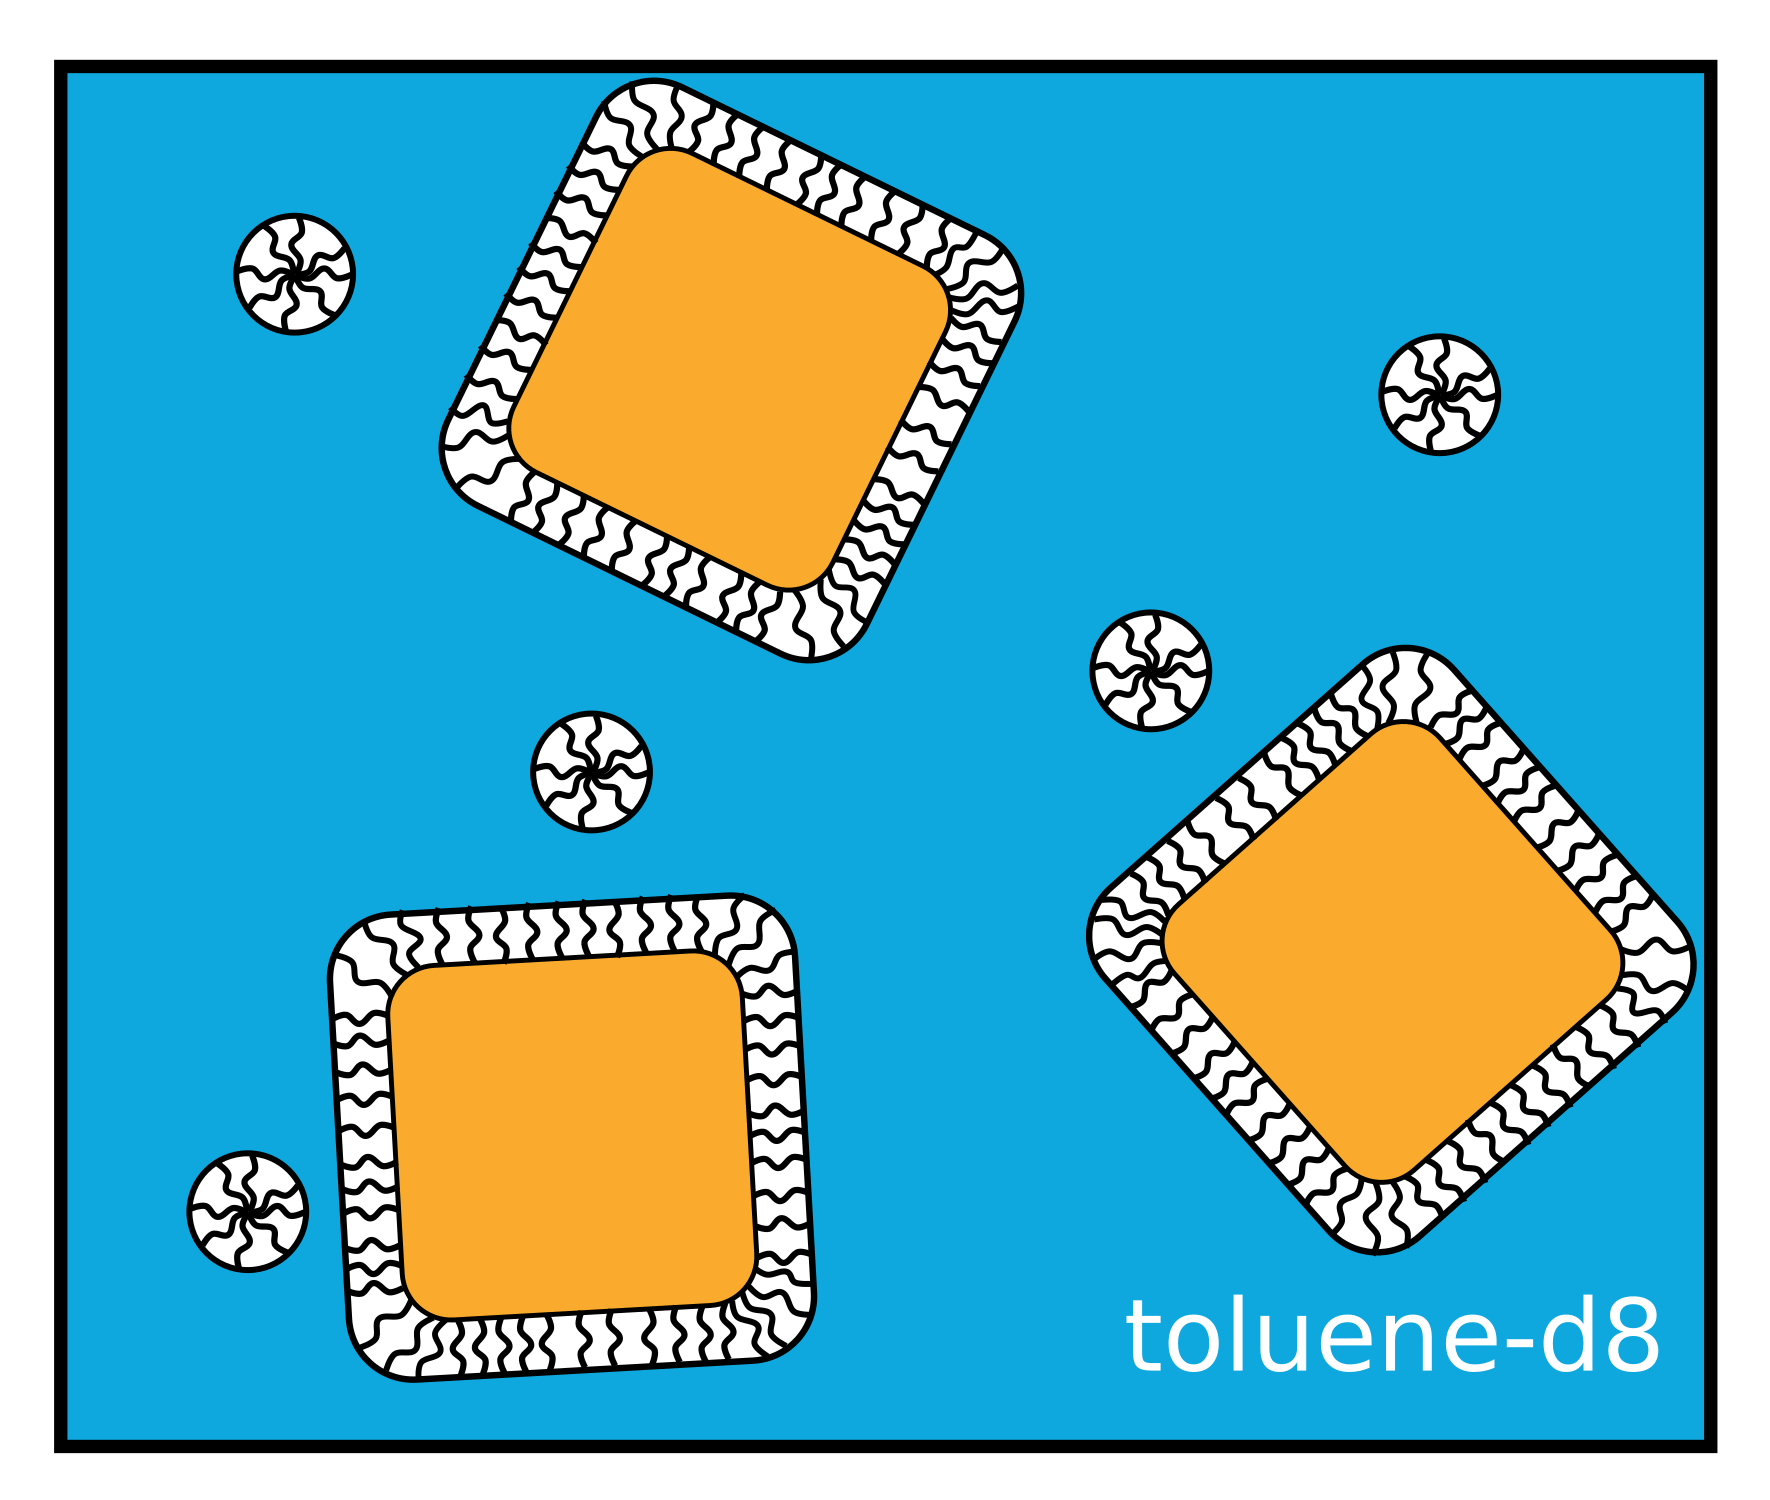
\includegraphics{monolayer_sans_superball_OA_model}
  %     \caption{\label{fig:monolayers:charMethods:SANSModel}Depiction of the model used for SANS: A combination of nanoparticles and oleic acid micelles. Orange is the nanoparticle material, white with curly lines the oleic acid and blue the solvent.}
  %   \end{figure}

  %   Due to the stronger contrast of oleic acid and the solvent for neutrons, oleic acid micelles in the solution become visible.
  %   Also it is possible that a incoherent background might be present due to the hydrogen of the oleic acid (\ch{C18H34O2}), as to why an additional constant background term is added to the model.
  %   The SANS data is thus described by a sum of the intensity calculated for the superball, the intensity of a spherical form factor and a constant term
  %   \begin{align}
  %     I(q) \eq I_\mathrm{superball}(q) + I_\mathrm{sphere}(q) + I_\mathrm{bg},
  %   \end{align}
  %   which is depicted in \reffig{fig:monolayers:charMethods:SANSModel}.
  %   The micelles introduce $r_\mathrm{OA}$ and $n_\mathrm{OA}$ as additional parameters to the model, which describe the size of the micelles and their number density in dispersion.

  %   To interpret particle number densities $n$, they are transformed to a mass concentration by
  %   \begin{align}
  %     c_m \eq n \rho V_p,
  %   \end{align}
  %   using the single-particle volume $V_p$ and the density of the material $\rho$.
  %   For the oleic acid micelles the volume fraction
  %   \begin{align}
  %     c_V \eq n V_p,
  %   \end{align}
  %   is given instead as it is the more natural to the liquid state of oleic acid.

  % \paragraphNewLine{Vibrating Sample Magnetometry}
  %   The macroscopic magnetization of the nanoparticles Ac-CoFe-C, Ac-CoFe-C-2 and Ol-CoFe-C was measured using the PPMS Evercool II described in \refch{ch:instruments:laboratoryInstruments:vsm}.
  %   To obtain the magnetization in a non-interacting state at room temperature, two approaches have been considered.
  %   In the first, $40 \unit{\musf L}$ of the nanoparticle dispersion are sealed in a vial as described in \refch{ch:instruments:laboratoryInstruments:vsm}.
  %   The vial is subsequently fixed within a drinking straw, using additional folded straws to render the vial immobile.
  %   A moving liquid sample is a difficult system in the framework of vibrating sample magnetometry as due to air gaps the liquid is still able to move within its container during the vibration, which can lead to a systematic error in the measured signal \cite{Boekelheide_2016_Artif}.
  %   Therefore, in a second approach, the nanoparticle dispersion is quickly drop casted in a diluted concentration ($c \eq 0.1 \unit{mg/mL}$) on a silicon substrate using $\textit{n}$-hexane as solvent to measure the nanoparticles in a dry state for comparison.
  %   The background of the silicon substrate and sample holder is subtracted in this case by the measurement of an empty silicon wafer with approximately the same mass.

  %   For both approaches hysteresis curves are measured at $10 \unit{K}$ and $300 \unit{K}$, as well as on five additional temperatures in between ($20\unit{K},\,50\unit{K},\,100\unit{K},\,150\unit{K},\,200\unit{K}$).
  %   Before each measurement, a touchdown procedure is performed with the sample rod, to correct for thermal expansion due to the temperature changes.
  %   Each hysteresis is measured in sweep mode with a rate of $5 \unit{mT \, s^{-1}}$.
  %   Additionally, for the dry particles on a substrate, zero-field-, field-cooled warming curves are measured at a field of $10 \unit{mT}$ for a temperature range from $10 \ldots 350 \unit{K}$ with a heating rate of $1.5 \unit{K \, min^{-1}}$.

  %   The scaling of the data to the volume of the sample is performed as described in \refch{ch:methods:vsm}:
  %   By fitting the room-temperature data to a Langevin behaviour plus a term for an excess susceptibility in the case of the nanoparticle dispersions, the magnetization data is scaled such that the saturation magnetization is given by the ratio of the single-particle moment and volume.
  %   \begin{align}
  %     M_s \eq \frac{\bar{\mu}}{V_p}.
  %   \end{align}
  %   The average particle volume and particle size distribution is hereby taken from the previously obtained SAXS data evaluation and the standard deviation of the magnetic moment is set to be three times the particle size distribution $\sigma_{\mu} \eq 3 \sigma_{a}$, assuming the magnetic moment scales proportionally with the volume.
\end{document}